\subsection{Hidden Markov Models: functional modelization}

\subsubsection{Context of Hidden Markov Models and Hidden Tree Markov Models}

One key goal of our analysis of the microbiota is to highlight functional groups of
bacteria in a studied context (reaction to treatment, overall view, disease tracking, post-surgery reaction, ...).
Unveiling such groups can be done through various processes, namely by using latent variables.

\medskip

Previously, we have worked with i.i.d latent variables, meaning that the hidden representation does not
implement any typical graph structure that would model latent dependencies between the bacteria (i.e., functional areas).
A typical latent model that would admit the simplest graph structure of a chain is given by the Hidden Markov Models.

\medskip

In a nutshell, Hidden Markov Models (HMM) are a class of generative models such that the latent variable follows a Markov Chain.
Formally, for an observed variable $Y = (Y_1, \dots, Y_n)$, $Z = (Z_1, \dots, Z_n)$ is a discrete HMM relatively to $Y$ if we have the following:
\begin{itemize}
    \item $Z$ is a Markov Chain (MC) with discrete states:
         $$
         \mathbb{P}(Z_{i+1} | Z_i, Z_{i-1}, \dots, Z_1) = \mathbb{P}(Z_{i+1} | Z_i)
         $$
    \item We define a prior on the seed of the MC:
         $$\forall c \in \{1, \dots, C\}, \mathbb{P}(Z_1 = c) = \pi_c$$

    \item We define a transition probability on the states of the MC:
        $$\forall c,k \in \{1, \dots, C\}^2, \mathbb{P}(Z_{i+1} = c | Z_i = k) = t_{k,c}^{(i+1)}$$

    \item We define an emission probability for $Y$ to be in a given state when observing $Z$:
        $$
        P(Y_i \in A | Z_i = c) = a_c(A)
        $$
\end{itemize}

\begin{figure}[H]
    \centering
    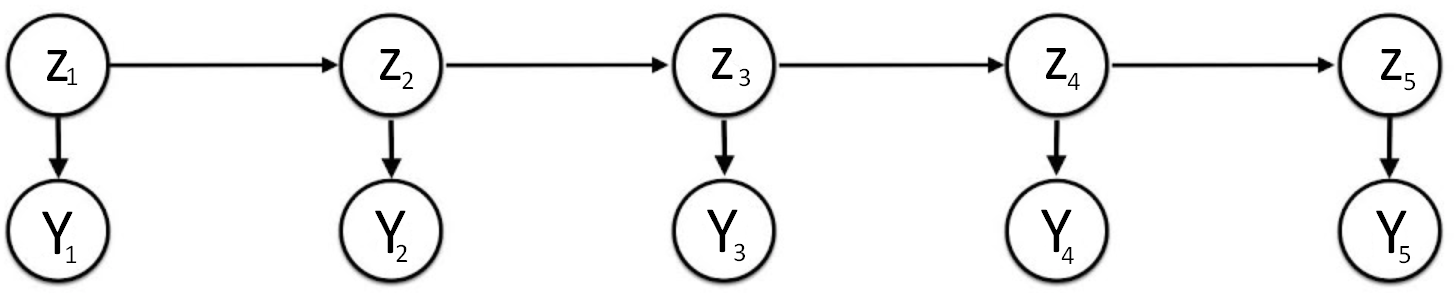
\includegraphics[scale=.25]{images/graph_dependency_HMM}
    \caption{Dependency graph of a HMM ($Z$ is the latent MC, $Y$ the observation)}
    \label{fig:graph_dependency_hmm}
\end{figure}

As a result, we can use HMM to model hidden functional groups of bacteria from one layer to the other.

This idea can even be extended to the specific tree-like structure of taxa-abundance data, introducing
the wider class of models given by the Hidden Tree Markov Model (HTMM) \cite{hidden_tree_markov_models}.
The HTMM provides a dependency graph that accounts for the tree structure, so that instead of a chain, we get
a Markov tree.
The following figure illustrates a given HTMM, precisely a top-down architecture:

\begin{figure}[H]
    \centering
    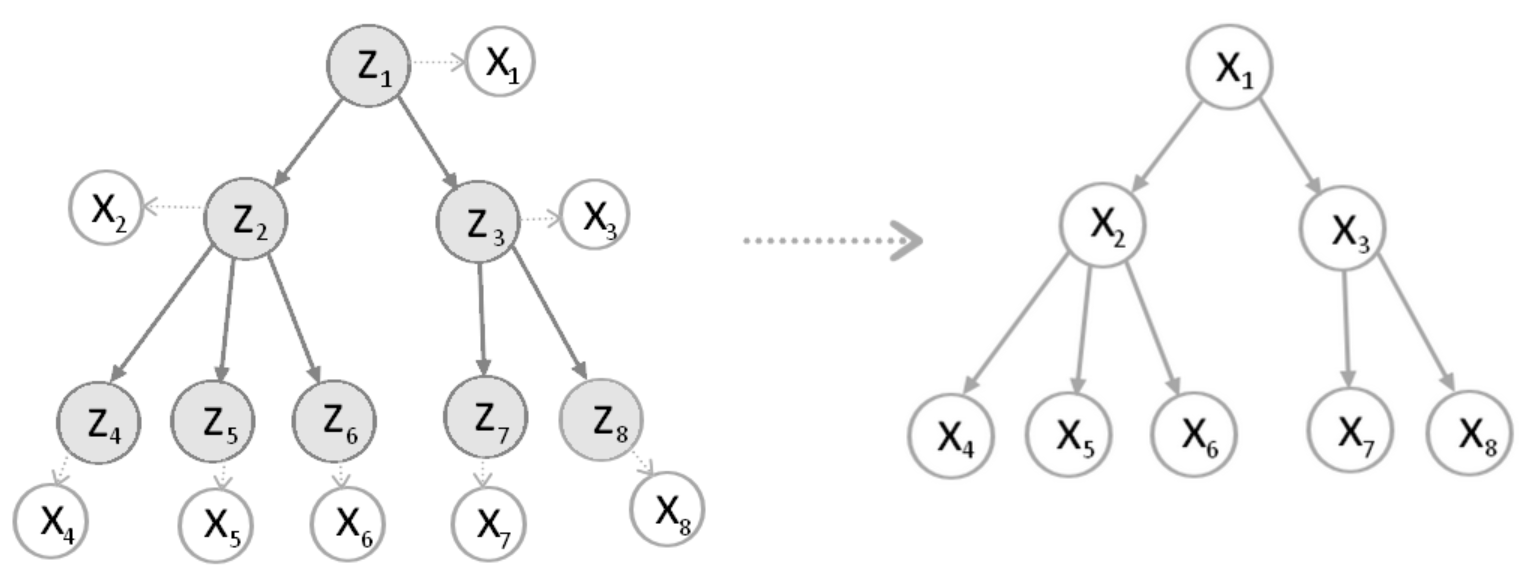
\includegraphics[scale=.5]{images/top_down_htmm_example}
    \caption{Top-down HTMM example: $Z$ represents the latent Markov tree,
        $X$ the observed abundance of a given bacteria in the taxonomic tree}
    \label{fig:top_down_htmm_example}
\end{figure}

The mathematical framework is then slightly different for top-down HTMM:
\begin{itemize}
    \item $Z$ is a Markov Tree (MT):
        $$\mathbb{P}\left(Z_{k}^{(l)} = c | Z_{0}^{(\ell)}, \dots, Z_{K_{\ell}}^{(\ell)}, \nodeparent(Z_{0}^{(\ell)}), \dots, \nodeparent(Z_{K_{\ell}}^{(\ell)}), \dots, Z_1^{(1)} \right) = \mathbb{P}\left(Z_{k}^{(\ell)} | \nodeparent(Z_{k}^{(\ell)})\right)$$
    \item We define a prior on the first layer of the MT, relatively to a given tree $T$:
        $$
        \mathbb{P}\left(Z_1^{(1)} = j | T^{(1)}\right) = a_j
        $$
    \item We define the transition probabilities of the MT, relatively to a given tree $T$:
        $$\mathbb{P}\left(\childrennode(Z_k^{(\ell)}) = \nu | Z_k^{(\ell)} = j, T^{(\ell+1)}\right) = t_{\nu,j}^{(\ell)}$$
\end{itemize}

Notice that this model would be tree dependent, as we want to attach existing nodes to a given hidden state, to generate
the abundance accordingly.
One could think of a tree generator model by applying the HTMM onto the global taxonomy directly, and defining an "empty"
state that would turn off the specific nodes in the final representation.

\medskip

Some recent work on HTMM have been showing that top-down modelling captures
less discriminent detail and conditional dependencies between the nodes than the bottom-up architecture \cite{bottom_up_superiority_hidden_tree_markov_models}.
However, taxa-abundance data constraints may not be compatible with a bottom-up approach,
as fixing the leaf nodes provides the whole information about the tree (structure and abundance).
Hence, in our specific use case, bottom-up trees are less likely to capture the latent structure of the trees
as it would only model the last layer.

\subsubsection{Tree generation: layer-wise Hidden Markov Model}

In this section, we aim at modeling the distribution of the trees $(T_i)_{1 \leq i \leq n}$ through a layer-wise Hidden Markov Model.
The following figure illustrates the dependency between the latent markov chain and the tree:
\begin{figure}[H]
    \centering
    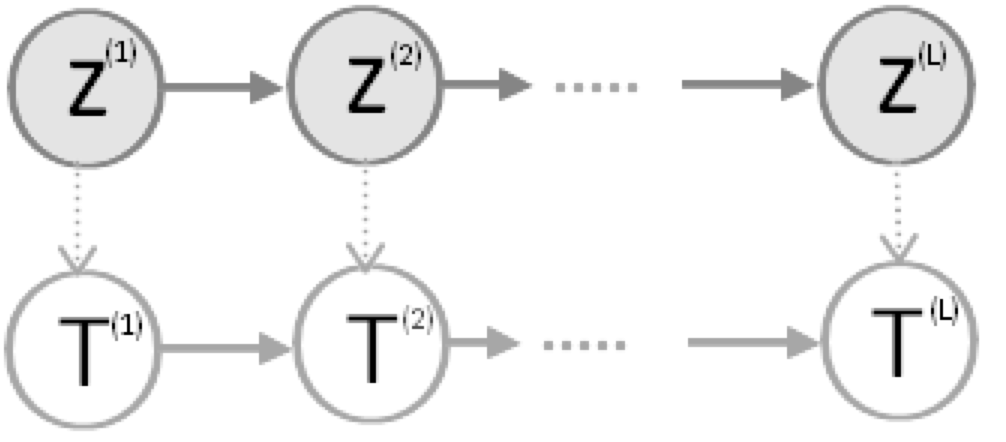
\includegraphics[scale=.4]{images/layer_wise_hidden_markov_model_tree}
    \caption{Layer-wise hidden markov model dependency graph: $Z$ is the HMM, $T^{(\ell)}$ is the layer $(\ell)$ of the tree}
    \label{fig:layer_wise_hmm_tree}
\end{figure}

As illustrated on figure \ref{fig:layer_wise_hmm_tree} and by nature of our taxonomic data,
the layer of the tree follow a Markov process (at least, it could be deeper than markovian).
Conversely to the previous situations, the latent variable now follows a markov chain as well, which enables to
group the layers of the tree with a dependence on the parent's layer group.

\medskip

Furthermore, in that approach, we decide to model the layers rather than the nodes to introduce dependency between
the nodes of a given layer, so we do not look into the $u_k^{(\ell)}$ anymore but directly into the $T^{(\ell)}$.

\medskip

Concisely, the mathematical framework can be written as follow:
\begin{itemize}
    \item $Z$ follows a discrete MC:
        $$
        \begin{align}
            &\mathbb{P}\left(Z^{(1)} = c\right) = a_c \\
            &\mathbb{P}\left(Z^{(\ell+1)} = k | Z^{(\ell)} = c\right) = t_{c,k}^{(\ell+1)}
        \end{align}
        $$
    \item $T$ is markovian and parameterized conditionally to $Z$.
          We denote by $\childrennode(T^{(\ell)})$ the set of plausible activation vectors at layer $(\ell+1)$ in the taxonomy, relatively to
          the parents activation given by $T^{(\ell)}$. We then model the emission probability by:
        $$\mathbb{P}(T^{(\ell+1)} = \omega | Z^{(\ell+1)} = c, T^{(\ell)}) = \frac{\pi_c(\omega) \mathds{1}_{\omega \in \childrennode(T^{(\ell)})}}{\sum_{\nu \in \childrennode(T^{\ell})} \pi_c(\nu)}$$

\end{itemize}

One may notice that such modelisation on $T$ will require a large number of parameters.
Indeed, the set of plausible activation vectors at layer $(\ell+1)$ relatively to $T^{(\ell)}$ can be quite big, as for each activate node $u_k^{(\ell)}$ in $T^{(\ell)}$
we get $2^{|\childrennode(u_k^{(\ell)})|} - 1$ plausible activated vectors of its children ($-1$ comes from the fact that we would like to avoid missing values).
We denote by $\mathcal{S}(Z)$ the discrete state space of the hidden markov chain.
Hence, for a given tree $T$, we obtain a total number of parameters of:
$$
n_{\text{params}} = \sum_{\ell=1}^{L}\sum_{k=1}^{K_{\ell}} |\mathcal{S}(Z)| \times \left(2^{|\childrennode(u_k^{(\ell)})|} - 1\right)
$$

As usual for latent data models, variational methods come in handy for learning the model.
Hence, we provide an Expectation-Maximization algorithm to compute the optimal parameters of the prior over the tree
in proposition ???.
The E-M algorithm can be summarized as follow:
\begin{itemize}
    \item \textbf{Expectation step}:
    \item \textbf{Minimization step}:
\end{itemize}

\subsubsection{Abundance generation: Hidden Tree Markov Model}

In this section, we aim at modeling the distribution of the abundance data $(X_i)_{1 \leq i \leq n}$ conditionally
to its known corresponding trees $(T_i)_{1 \leq i \leq n}$, using a Hidden Tree Markov Model (HTMM).
The dependency graph is illustrated by the figure \ref{fig:top_down_htmm_example}, giving us the follow mathematical framework:

\begin{itemize}
    \item $Z$ is a discrete Markov Tree (MT):
        \begin{itemize}
            \item We define a prior over the root:
                $$\mathbb{P}(Z_1^{(1)} = c | T^{(1)}) = a_j$$
            \item We define the transition probabilities:
                $$\mathbb{P}(\childrennode(Z_k^{(\ell)}) = \nu | Z_k^{(\ell)} = j, T^{(\ell+1)}) = t_{j,\nu}^{(\ell)}$$
        \end{itemize}
    \item $X$ follows a Markov Tree structure.
        We define the emission probability of the corresponding abundance relatively to the hidden states and tree:
        $$p(\childrennode(x_k^{(\ell)}) | \childrennode(Z_k^{(\ell)}) = \nu, x_k^{(\ell)}, T^{(\ell+1)}) \sim x_k^{(\ell)} \mathcal{D}(\alpha_{\nu,k}^{(\ell)} \odot T^{(\ell+1)}_k)$$
\end{itemize}

The number of parameters of that model is quite large, as it depends on the size of the latent space state and the number of child node
of each parent node in the tree structure.
Indeed, for each node, the corresponding dirichlet parameter is of the size of the number of children (if it has more than 1 child).
Then, we have as many dirichlet parameters as the possible amount of vector $\nu$, for which each coordinate has $|\mathcal{S}(Z)|$ plausible value.
That leads us to the following number of parameters:
$$
n_{\text{params}} = \sum_{\ell=1}^L \sum_{k=1}^{K_{\ell}} |\mathcal{S}(Z)|^{|\childrennode(u_k^{(\ell)})|} \times |\childrennode(u_k^{(\ell)})| \times \mathds{1}_{|\childrennode(u_k^{(\ell)})| > 1}
$$

As previously for the tree generation, we propose an Expectation-Maximization algorithm to compute the optimal parameters of
that HTMM, detailed in proposition ???. The E-M sums up as follows:
\begin{itemize}
    \item \textbf{Expectation step}:
    \item \textbf{Maximization step}:
\end{itemize}